\documentclass[10pt,a4paper]{article}
\usepackage[utf8]{inputenc}
\usepackage{fancyhdr}
\usepackage[spanish]{babel}
\usepackage{amsmath}
\usepackage{amsfonts}
\usepackage{amssymb}
\usepackage{lastpage}
\usepackage[left=2.5cm,right=2.5cm,top=2.75cm,bottom=2.5cm]{geometry}
\usepackage{graphicx}
\usepackage{hyperref}
\hypersetup{
    colorlinks,
    citecolor=black,
    filecolor=black,
    linkcolor=black,
    urlcolor=black
}


\setlength{\headheight}{25pt}
\fancyhf{} % sets both header and footer to nothing
\renewcommand{\headrulewidth}{0pt}
\fancyhead[LO,RE]{
    		\centering
    		\begin{tabular}{|c|l|l|}
    			\hline
   		 		\textbf{EN} & \textit{Análisis de riegos de la gestión de la configuración en un TFG} & 23/04/2017 \\\cline{2-3} 
    			\textbf{SO} & \multicolumn{2}{|c|}{\textbf{DOC: p7\_riesgosTFG.pdf}}   \\ \hline
    		\end{tabular}
              }
\cfoot{Página \thepage\ de \pageref{LastPage}}
\author{Canosa Domínguez, Cristofer \\ Rodríguez Alcaraz, Silvia \\ Seijas Salinas, Orquídea Manuela \\ Soutullo Sobral, Samuel}
\title{Análisis de riegos de la gestión de la configuración en un TFG}

\begin{document}
	\maketitle %TODO poner portada bonita
	\newpage
	\begin{table}[htb]
    	\centering
    	\begin{tabular}{|l|l|l|}
   			\hline
    		\multicolumn{3}{|c|}{CONTROL DE VERSIONES} \\ \hline
    		VERSIÓN & FECHA & DESCRIPCIÓN DEL CAMBIO\\
    		\hline \hline
    		1.0 & 07/04/2017 & Creación del documento \\ \hline
    	\end{tabular}   
    \end{table}
	\newpage
	\tableofcontents
	\newpage
	\pagestyle{fancy}
	\section{Descripción de la práctica}
	La práctica que recoge este documento consiste en la realización del proceso completo de gestión de riesgos sobre el desarrollo de un Trabajo de Fin de Grado. Cabe destacar que tan sólo se contemplan los riesgos que están relacionados con la gestión de la configuración.\\
	
	El procedimiento a seguir ha sido, en primer lugar, la identificación de activos dentro del proyecto planteado. Con activos nos referimos tanto a los elementos de configuración, como a las líneas base, el sistema de gestión de la configuración y el proceso. Por otra parte, también fueron identificadas las fuentes de riesgo para poder proceder al análisis de riesgos.\\
	
	El análisis de riesgos, por su parte, se basó en la identificación de los mismos en función de los activos previamente definidos para, finalmente, poder llevar a cabo una planificación donde se plantean acciones de prevención y  minimización. Para los riesgos más importantes, se ha planteado realizar un seguimiento a lo largo del trabajo de fin de grado. La fecha utilizada para observar cada uno de los riesgos ha sido seleccionada de la planificación propuesta sobre un TFG que viene en las transparencias del enunciado. Dicha propuesta, se recoge en el siguiente diagrama de Gantt. \\
	
	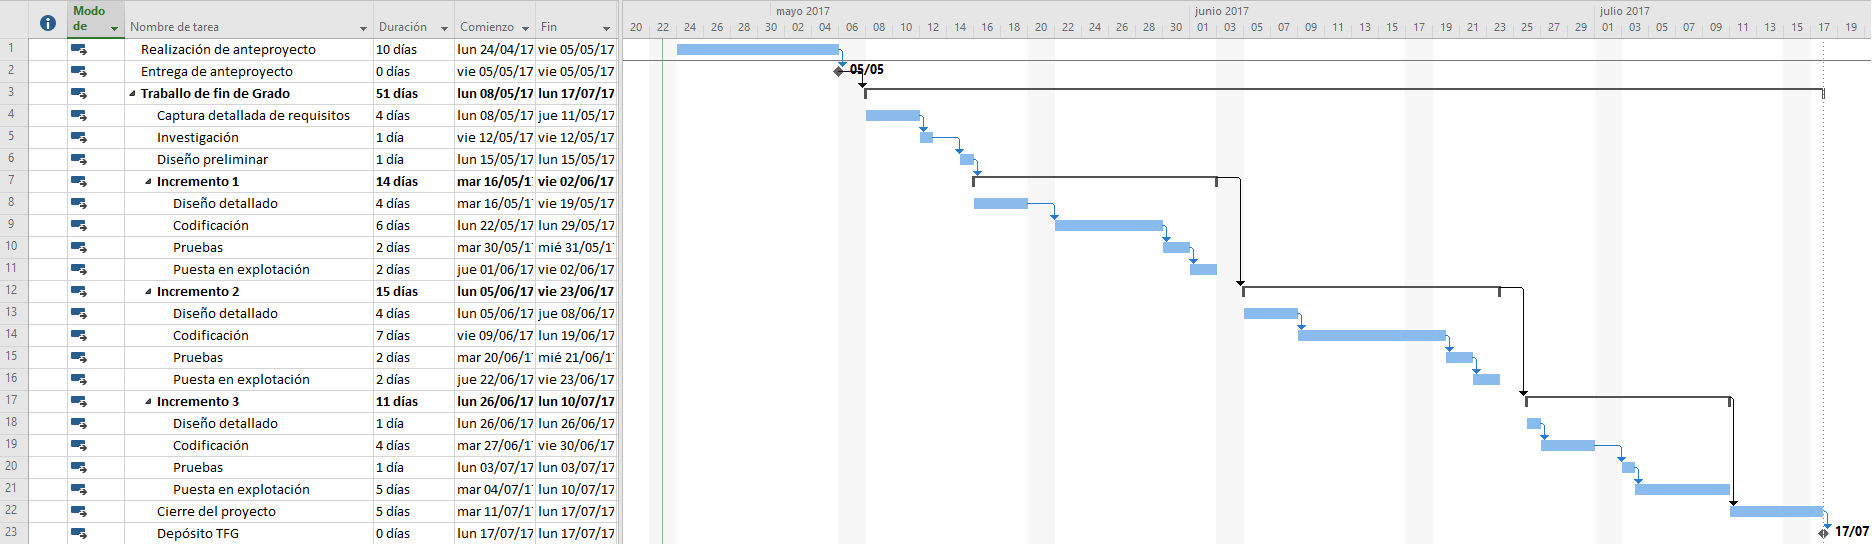
\includegraphics[scale=0.3]{imagenes/tfg.png}
		
	\section{Descripción del grupo de trabajo}
		\begin{table}[htb]
        \centering
        \begin{tabular}{|l|l|l|}
        \hline
        \multicolumn{2}{|c|}{\textbf{Grupo de trabajo}} \\ \hline
       \textbf{Nombre} & \textbf{Rol}\\
        \hline \hline
        Crístofer Canosa Domínguez & Validador de requisitos \\ \hline
        Silvia Rodríguez Alcaraz & Aseguradora de calidad \\ \hline
        Orquídea Seijas Salinas & Gestora documental \\ \hline
        Samuel Soutullo Sobral & Jefe de proyecto \\ \hline
        \end{tabular}   
        \end{table}
		
	\section{Planificación de la práctica}
		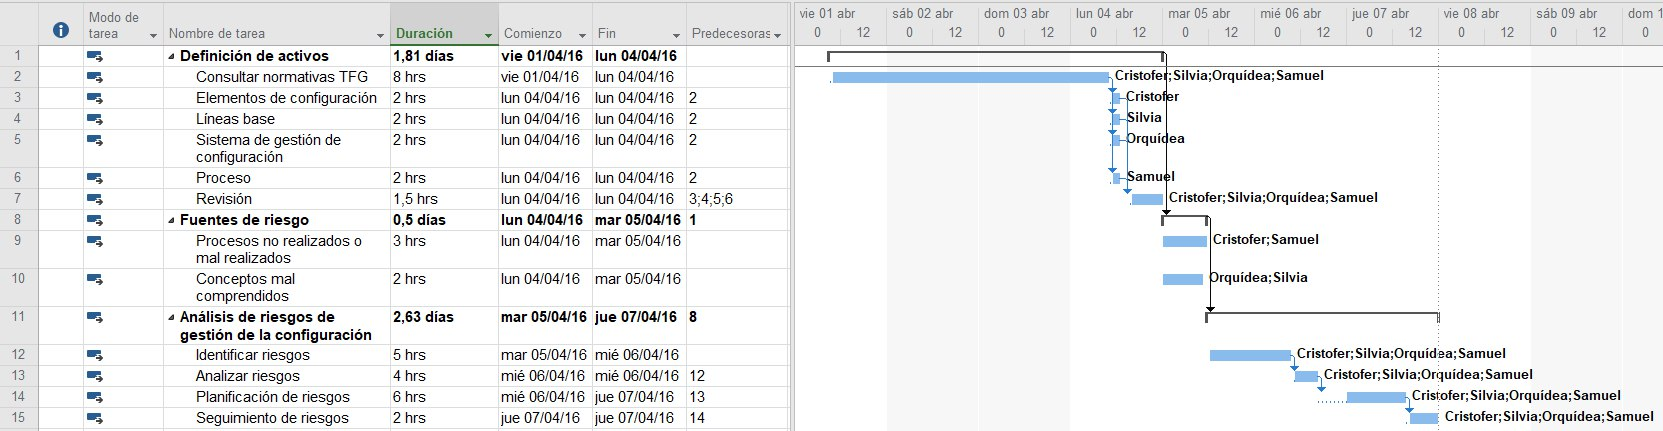
\includegraphics[scale=0.25]{imagenes/planificacion.jpg}
		
	\section{Desarrollo de la práctica}
		\subsection{Identificación de activos}
			\subsubsection{Elementos de configuración} 
			\begin{itemize}
                \item Solicitud de anteproyecto: Supone una entrega formal donde, además, se exponen datos concretos sobre la implementación del trabajo (propuesta de solución, planificación, etc).
                \item Documento de análisis: Estudio de requisitos del trabajo, junto a una planificación temporal y análisis de costes.
                \item Documento de diseño: Conjunto de diagramas y documentos anexos donde se define el diseño a implementar en la entrega.
                \item Repositorio de código: Conjunto de archivos fuente y de configuración necesarios para construir la aplicación.
                 \item Repositorio de documentación: Páginas, libros y otros documentos consultados para la realización del trabajo. Es conveniente guardarlos localmente para mantener la versión visitada en caso de que la versión online se actualice o desaparezca.
                 \item Presentación del trabajo: Incluye la memoria y el documento de la presentación oral, que serán un aglomerado del resto de documentos que componen el trabajo.
                 \item Manuales técnicos y de usuario: El manual técnico contiene información sobre la implementación de la                         aplicación para su posterior ampliación o modificación por parte de terceros. El manual de usuario funciona como guía para usuarios comunes del programa.
            \end{itemize}
			\subsubsection{Líneas base}
				\begin{itemize}
			    	\item Solicitud: El producto de esta etapa sería la propia solicitud de TFG. Una vez aprobada la solicitud del alumno, éste puede pasar a la siguiente etapa del proceso sin modificaciones sobre esta propuesta. Es decir, en principio, debe continuar con el trabajo presentado.
			    	\item Análisis y diseño: En esta etapa el alumno realizará los pertinentes estudios para establecer tanto los requisitos y costes del trabajo como los diagramas pertinentes que describan el sistema a implementar. Los productos de esta etapa serán el documento de análisis y el de diseño, los cuales deberán ser aprobados para proceder a la implementación. Una vez aprobados, los productos no podrán ser modificados sin emplear un proceso de control de cambios estricto.
			   	 	\item Implementación: El producto de esta etapa será el código de la aplicación a desarrollar. Este código debe ser plenamente funcional y cumplir tanto con la estructura descrita en el diseño como con los requisitos determinados en el análisis para ser aprobado.
			   		\item Documentación: Los productos son la memoria del proyecto, el documento de presentación oral y los manuales técnicos y de usuario. Todos los documentos deben ser claros, precisos y completos para asegurar su aprobación. Esta sería la última etapa del proceso, una vez finalizada éste debería haberse completado. La comparación de las distintas líneas base permitirá comprobar si los tiempos estimados para cada etapa se han cumplido o no y, en este caso, cómo se han desviado de la planificación inicial.	    			    
				\end{itemize}
			\subsubsection{Sistema de gestión de configuración}
			\begin{itemize}
			    \item Git: Se ha decidido utilizar Git como sistema de gestión de configuración, puesto que al ser un proyecto estrechamente relacionado con la implementación de código, es altamente probable que sea necesario registrar cada cambio realizado. Esta herramienta permitirá realizar esta actividad de manera rápida y eficiente, además de permitir el acceso a la lista de cambios fácilmente.
			\end{itemize}
			\subsubsection{Proceso}
			\begin{itemize}
			    \item Documentación de cambios: Conjunto de documentos creados con la finalidad de realizar un correcto seguimiento del control de cambios. Cobran especial importancia cuando se trata de cambios cuya introducción se ve forzada por causas externas al estudiante y afectan al trabajo ya realizado.
			    \item Documento de despliegue: Documento en el que se especifica de manera formal y clara los pasos a seguir para poder ejecutar la posible aplicación en cualquier equipo o conjunto de equipos que cumplan los requisitos necesarios para la ejecución de dicha aplicación.
			    \item Documento de validación: Documento generado como consecuencia de la realización de procesos de validación. Los procesos de validación determinan si el software final cumple o no los requisitos exigidos.
			    \item Software de entorno de desarrollo: Conjunto de todo el software necesario durante la fase de desarrollo. Esto incluye editores de texto, entornos de desarrollo integrados (IDE), compiladores, intérpretes, librerías, frameworks, etc.
                \item Computador de desarrollo: Máquina o máquinas usadas por el estudiante para la realización del trabajo durante todas las posibles fases del mismo (análisis, diseño, implementación, ...).	    
			    \item Computador de despliegue: Máquina o máquinas sobre las que se ejecutará finalmente el software en el momento en el que será evaluado por parte del tribunal.
			\end{itemize}
		\subsection{Identificación de fuentes de riesgo}
			\subsubsection{Retraso en el proceso de documentación (ISO 12207 - Soporte)}
			La documentación del proyecto se debe realizar al mismo tiempo que el trabajo en sí. De esta forma todo el proceso quedará especificado de forma permanente, evitando que en un punto posterior o en la memoria final se produzcan incoherencias entre lo que se especifica en la documentación y el producto final.
			\subsubsection{Nulo o deficiente proceso de validación (ISO 12207 - Soporte)}
			Si la lista de requisitos es muy amplia es conveniente automatizar de alguna forma su validación, por ejemplo, haciendo tests. 
No llevar un registro concreto de validación puede desembocar en una entrega incompleta.
			\subsubsection{No reevaluar los riesgos con cierta periodicidad (ISO 15504-2 - Gestión del Riesgo)}
			Para asegurar que se cumple la planificación establecida es conveniente reevaluar los riesgos con cierta periodicidad para evitar que surjan nuevos riesgos, así como para reducir el tiempo necesario para su gestión (en el caso de que algún riesgo ya no sea relevante).
		\subsection{Análisis de riesgos}
			\subsubsection{Riesgo R001: No tener en cuenta el tiempo disponible para la realización del anteproyecto}
				\paragraph{Probabilidad} Moderada
				\paragraph{Impacto}	Catastrófico
				\paragraph{Descripción} El hecho de que falte algún apartado o existan errores en la realización del documento puede hacer que se rechace por parte de la comisión de TFG. Por lo tanto, se debe organizar el tiempo para realizar todos y cada uno de los elementos obligatorios.
				\paragraph{Fecha} A lo largo del mes de marzo %Cuando puede producirse el riesgo. Ver el Gantt de Rabenso
				\paragraph{Tratamiento} Prevención %Minimización o prevención
				\paragraph{Acción} Se debe mantener un ECS con la planificación en la que estén definidos todos los elementos obligatorios y el tiempo disponible para su realización. La estimación del tiempo se puede revisar a lo largo de la realización del anteproyecto, pero siempre ajustándose a la fecha límite de entrega. %Descripción del tratamiento
				\paragraph{Indicadores} Alguno de los elementos está tardando más de lo debido conforme a la planificación. %Que nos puede indicar que se está produciendo el riesgo
				\paragraph{Seguimiento}	Semanal %Desde cuando empezar a seguir el riesgo. Este apartado solo aparece en riesgos con impactos altos.
	
            \subsubsection{Riesgo R002: No identificar correctamente los objetivos del trabajo}
				\paragraph{Probabilidad} Moderada
				\paragraph{Impacto}	Serio
				\paragraph{Descripción} Unos objetivos poco claros pueden llevar a la realización de trabajo innecesario, poco concreto, etc. Los objetivos deben estar correctamente establecidos para tenerlos siempre en cuenta a lo largo del proyecto.
				\paragraph{Fecha} 20/03/2017-30/03/2017 %Cuando puede producirse el riesgo. Ver el Gantt de Rabenso
				\paragraph{Tratamiento} Minimización %Minimización o prevención
				\paragraph{Acción} Definición de los objetivos en un ECS y revisión de los mismos con el tutor asignado. %Descripción del tratamiento
				\paragraph{Indicadores} No se tiene claro el proceso a seguir en alguna de las fases de realización del trabajo. %Que nos puede indicar que se está produciendo el riesgo
				\paragraph{Seguimiento}	Cuando el indicador aparece. %Desde cuando empezar a seguir el riesgo. Este apartado solo aparece en riesgos con impactos altos.	
				
			\subsubsection{Riesgo R003: Identificar incorrectamente los requisitos del trabajo }
				\paragraph{Probabilidad} Alta
				\paragraph{Impacto}	Serio
				\paragraph{Descripción} Una mala identificación de los requisitos puede llevar a plantear una solución incorrecta, poco definida, etc. Esto puede implicar el rechazo de la solicitud.
				\paragraph{Fecha} 20/03/2017-30/03/2017 %Cuando puede producirse el riesgo. Ver el Gantt de Rabenso
				\paragraph{Tratamiento} Prevención %Minimización o prevención
				\paragraph{Acción} Aumentar el tiempo necesario para la especificación de los requisitos, siendo posible profundizar en el diseño para encontrar errores de forma temprana. %Descripción del tratamiento
				\paragraph{Indicadores} Un planteamiento de solución no cumple con la definición de los objetivos. %Que nos puede indicar que se está produciendo el riesgo
				\paragraph{Seguimiento}	Semanal %Desde cuando empezar a seguir el riesgo. Este apartado solo aparece en riesgos con impactos altos.
				
			\subsubsection{Riesgo R004: No conseguir ajustar la planificación a las horas requeridas }
				\paragraph{Probabilidad} Alta
				\paragraph{Impacto}	Tolerable
				\paragraph{Descripción} El trabajo debe ocupar unas horas establecidas para ser válido. En caso de no cumplirlas se debe exponer una razón adecuada.
				\paragraph{Fecha} 20/03/2017-30/03/2017
				\paragraph{Tratamiento} Prevención %Minimización o prevención
				\paragraph{Acción} Una vez realizada la planificación, si no cumple con las restricciones temporales establecidas, habrá que replantearse los requisitos para ampliarlos o disminuirlos.  %Descripción del tratamiento
				\paragraph{Indicadores} La planificación no cumple con las restricciones temporales establecidas. %Que nos puede indicar que se está produciendo el riesgo
				
			\subsubsection{Riesgo R005: Inhabilidad para estimar los costes del trabajo}
				\paragraph{Probabilidad} Moderada
				\paragraph{Impacto}	Tolerable
				\paragraph{Descripción} Se debe realizar una estimación de coste de todo el proyecto previa a su desarrollo.
				\paragraph{Fecha} 20/03/2017-30/03/2017 %Cuando puede producirse el riesgo. Ver el Gantt de Rabenso
				\paragraph{Tratamiento} Minimización %Minimización o prevención
				\paragraph{Acción} Realizar la estimación después de un diseño suficientemente profundo de la solución. De ser necesario, se recurre a ayuda externa. %Descripción del tratamiento
				\paragraph{Indicadores} El coste es desproporcionado con respecto a implementaciones similares. %Que nos puede indicar que se está produciendo el riesgo
				
			\subsubsection{Riesgo R006: Errores a la hora de establecer las herramientas que se usarán para el desarrollo del proyecto}
				\paragraph{Probabilidad} Moderada
				\paragraph{Impacto}	Serio
				\paragraph{Descripción} Todas las herramientas deben establecerse desde un inicio para evitar incompatibilidades entre ellas o con la implementación en sí.
				\paragraph{Fecha} 20/03/2017-30/03/2017 %Cuando puede producirse el riesgo. Ver el Gantt de Rabenso
				\paragraph{Tratamiento} Prevención %Minimización o prevención
				\paragraph{Acción} Realizar un estudio de todas las herramientas a usar, así como un proyecto de prueba para su interoperabilidad. Además, se mantendrán como ECS todas las versiones usadas para que la versión utilizada sea recuperable y transferible en cualquier momento. %Descripción del tratamiento
				\paragraph{Indicadores} Errores en las pruebas de integración. %Que nos puede indicar que se está produciendo el riesgo
				\paragraph{Seguimiento}	Al finalizar cada incremento. %Desde cuando empezar a seguir el riesgo. Este apartado solo aparece en riesgos con impactos altos.
				
			\subsubsection{Riesgo R007: Diseño poco concreto que pierda su utilidad}
				\paragraph{Probabilidad} Moderada
				\paragraph{Impacto}	Serio
				\paragraph{Descripción} Si no se especifican comportamientos concretos es probable que se diseñen módulos que no funcionan o se olviden requisitos. Se debe documentar el diseño en la medida posible.
				\paragraph{Fecha} Cuando se realice el diseño detallado de cada incremento: 08/04/17-13/04/17, 28/04/17-04/05/17, 19/05/17.%Cuando puede producirse el riesgo. Ver el Gantt de Rabenso
				\paragraph{Tratamiento} Minimización  %Minimización o prevención
				\paragraph{Acción} Es necesario corregir el diseño, con el consiguiente retraso que conlleve respecto a la planificación del TFG. Es posible que no sea posible cubrir los requisitos más superficiales de la aplicación.%Descripción del tratamiento
				\paragraph{Indicadores} En el momento en el que se realiza el módulo de implementación, no se sigue el diseño inicial, ya que no cumple con todos los requisitos necesarios. %Que nos puede indicar que se está produciendo el riesgo
				\paragraph{Seguimiento}	En el momento en el que se empiece a codificar y hasta que se acabe de manera satisfactoria, se realizará un seguimiento diario. %Desde cuando empezar a seguir el riesgo. Este apartado solo aparece en riesgos con impactos altos.
			
			\subsubsection{Riesgo R008: Errores en el despliegue de la aplicación}
				\paragraph{Probabilidad} Bajo
				\paragraph{Impacto}	Serio
				\paragraph{Descripción} Se producen errores graves en la implementación de la aplicación por no tener un diseño claro y un conocimiento amplio de las herramientas a utilizar.
				\paragraph{Fecha} Cuando se realice la codificación de cada incremento:14/04/17-26/04/17, 05/05/17-18/05/17, 20/05/17-27/05/17. %Cuando puede producirse el riesgo. Ver el Gantt de Rabenso
				\paragraph{Tratamiento} Prevención %Minimización o prevención
				\paragraph{Acción} Completar cada módulo y realizar las pruebas necesarias sobre el mismo antes de implementar el siguiente. Así, cada módulo completo será plenamente funcional y los errores serán más fáciles de detectar y corregir porque estarán en un módulo completo%Descripción del tratamiento
				\paragraph{Indicadores} Que una prueba relacionada con el módulo falle.  %Que nos puede indicar que se está produciendo el riesgo
				\paragraph{Seguimiento}	Cada vez que se realice una prueba. %Desde cuando empezar a seguir el riesgo. Este apartado solo aparece en riesgos con impactos altos.
								
			\subsubsection{Riesgo R009: Desactualización del repositorio de documentación}
				\paragraph{Probabilidad} Baja
				\paragraph{Impacto}	Serio
				\paragraph{Descripción} La desactualización del repositorio supondría altas probabilidades de perder la documentación realizada hasta el momento, creando inconsistencias en el proyecto debido a la falta de información crucial. 
				\paragraph{Fecha} Construcción del repositorio (30/03/2017), actualizaciones después de cada uno de los 3 incrementos y actualización final el 09/06/2017 al finalizar el proyecto.
				\paragraph{Tratamiento} Prevención
				\paragraph{Acción} Después de cada punto crítico (ver fechas citadas) se revisará arduamente el repositorio de documentación comprobando que contiene todos los documentos generados en ese punto del proyecto.	Llevando a cabo estas acciones, al final del desarrollo el repositorio debería estar completo.			
				\paragraph{Indicadores} Consultas no exitosas de la documentación, es decir, no encontrar la información que se iba a buscar al repositorio.
				\paragraph{Seguimiento}	Desde el inicio del proyecto (30/03/2017) hasta el fin del mismo (09/06/2017)
				
			\subsubsection{Riesgo R010: Mal planteamiento en la presentación del trabajo}
				\paragraph{Probabilidad} Baja
				\paragraph{Impacto}	Tolerable
				\paragraph{Descripción} Su mal planteamiento puede provocar que no se entienda lo que ha sido desarrollado en el trabajo. 
				\paragraph{Fecha} Cierre del proyecto (04/06/2017-09/06/2017)
				\paragraph{Tratamiento} Prevención
				\paragraph{Acción} Plantear cuidadosamente la presentación del trabajo para no dejar ningún cabo suelto que pueda jugar en contra del autor a la hora de exponerlo. Además, realizar varias presentaciones de ser necesario realizando ensayos previos a la exposición.
				\paragraph{Indicadores} Incoherencias a la hora de tratar de exponer el trabajo.					

			\subsubsection{Riesgo R011: Presentación incompleta del trabajo}
				\paragraph{Probabilidad} Baja
				\paragraph{Impacto}	Catastrófico
				\paragraph{Descripción} La falta de contenidos en la presentación puede deberse a una mala gestión de cambios previa y, en este punto, generará inconsistencias al exponer el trabajo.
				\paragraph{Fecha} Cierre del proyecto (04/06/2017-09/06/2017)
				\paragraph{Tratamiento} Minimización
				\paragraph{Acción} En este punto del desarrollo tan sólo se puede revisar si los contenidos que faltan se han traspapelado o tratar de completarlos de la mejor forma posible antes de la exposición.
				\paragraph{Indicadores} Inconsistencia a la hora de exponer el trabajo debido a la falta de documentos o información.
				\paragraph{Seguimiento}	Este riesgo está muy ligado al R009, con tal de asegurar que el repositorio de documentación y el de código están actualizados en todo momento, no debería llegarse a este punto. Por esto, de no ser así el impacto es muy elevado pero la probabilidad de que ocurra baja ya que depende de dos riesgos ya estudiados.			
				
			\subsubsection{Riesgo R012: Incorrectas especificaciones en el manual técnico y de usuario}
				\paragraph{Probabilidad} Moderada
				\paragraph{Impacto}	Serio
				\paragraph{Descripción} La incorrecta especificación del manual de usuario llevaría al individuo que lo consulta a cometer errores en base a las especificaciones incorrectas. Además, los fallos a la hora de especificar el manual técnico podrían provocar errores fatales de cara al futuro ya que no reflejaría la realidad de la aplicación. Así, ésta podría ser tratada de un modo no apropiado.
				\paragraph{Fecha} Cierre del proyecto (04/06/2017-09/06/2017)
				\paragraph{Tratamiento} Prevención
				\paragraph{Acción} Realización de los manuales en base a toda la documentación actualizada y recopilada a lo largo del proyecto. Además, llevar a cabo varias reviosiones intensivas de los manuales en busca de falta de información, incongruencias o datos erróneos. Como método a mayores, dejar probar la aplicación a un usuario dejándole únicamente el manual de usuario como ayuda y recoger sus impresiones mediante un cuestionario a medida.
				\paragraph{Indicadores} 
				\begin{itemize}
				    \item Los usuarios no interactúan correctamente con la aplicación a pesar de consultar el manual de usuario.
				    \item Mediante el manual técnico es imposible rehacer idénticamente la aplicación.
				\end{itemize}				 
				\paragraph{Seguimiento}	Inicio del cierre del proyecto (cuando se empiezan a generar los manuales).
				
			\subsubsection{Riesgo R013. Inicio prematuro del TFG}
				\paragraph{Probabilidad} Baja
				\paragraph{Impacto}	Serio
				\paragraph{Descripción} Supondría comenzar a desarrollar el TFG antes de que el anteproyecto sea aprobado, pudiendo ser rechazado y perdiendo todo el progreso realizado.
				\paragraph{Fecha} A partir del 30/03/2017, cuando es entregado el anteproyecto.
				\paragraph{Tratamiento} Prevención
				\paragraph{Acción} Aguardar a la aprobación del anteproyecto para comenzar a trabajar en el proyecto.
				\paragraph{Indicadores} Falta de aprobación del anteproyecto.
				\paragraph{Seguimiento}	Período de tiempo posterior a la entrega del anteproyecto, donde se aguardará por su evaluación.
				
			\subsubsection{Riesgo R014: Análisis incorrecto de requisitos y diseño aprobados}
				\paragraph{Probabilidad} Moderada
				\paragraph{Impacto}	Catastrófico (peor de los casos)
				\paragraph{Descripción} El análisis incorrecto de requisitos y diseño del proyecto han sido considerados como lo suficientemente correctos como para pasar a la siguiente fase, por lo que el resto del proyecto se verá afectado. Por supuesto, esto dependerá de la gravedad del error cometido pero en el peor de los casos se tratará de un problema serio que podría retrasar la entrega del TFG.
				\paragraph{Fecha} 30/03/2017-14/04/2017. Desde que se inicia el trabajo hasta que comienza el primer incremento.
				\paragraph{Tratamiento} Prevención
				\paragraph{Acción} Revisión intensiva de los requisitos recogidos y el diseño realizado en busca de inconsistencias o a nivel de diseño y falta de requisitos. El diseño será refinado en los siguientes incrementos, por lo que el nivel de detalle no es crucial, pero sí que cumpla los requisitos expuestos.
				\paragraph{Indicadores} 
				    \begin{itemize}
				        \item Inconsistencias entre diseño y requisitos
				        \item Falta de requisitos en base a las especificaciones del cliente.
				        \item Problemas en posteriores fases del proyecto por el mal planteamiento del diseño y la falta de requisitos.
				    \end{itemize}
				\paragraph{Seguimiento}	La estrategia de prevención debe llevarse a cabo desde que se inicia el TFG hasta que comienza el primer incremento. A partir de este punto, si se han realizado correctamente las revisiones, ni los requisitos ni el diseño base deberían ser modificados. 

			\subsubsection{Riesgo R015: Validación de requisitos funcionales superficial}
				\paragraph{Probabilidad} Baja
				\paragraph{Impacto}	Serio
				\paragraph{Descripción} Una validación de requisitos funcionales superficial puede permitir que se entregue un software con una calidad mucho menor de la necesaria debido a falta de funcionalidades necesarias implementadas, por lo que se pondría en peligro el proyecto. 
				\paragraph{Fecha} Se puede producir cuando se realice la captura detallada de requisitos 30/03/17-05/04/17. %Cuando puede producirse el riesgo. Ver el Gantt de Rabenso
				\paragraph{Tratamiento} Prevención %Minimización o prevención
				\paragraph{Acción} Realizar la captura detallada de requisitos y consultarla con el tutor del TFG detalladamente para validarlos. %Descripción del tratamiento
				\paragraph{Indicadores} Requisitos funcionales definidos vagamente: un mismo requisito puede dar pie a que se interprete su funcionalidad de varias formas. %Que nos puede indicar que se está produciendo el riesgo
				\paragraph{Seguimiento}	Una vez se detecta el indicador del riesgo. %Desde cuando empezar a seguir el riesgo. Este apartado solo aparece en riesgos con impactos altos.
			
			\subsubsection{Riesgo R016: Documentación con errores ortográficos, gramaticales y sintácticos}
				\paragraph{Probabilidad} Baja
				\paragraph{Impacto}	Tolerable
				\paragraph{Descripción} Un documento que no se entienda, es muy difícil de valorar apropiadamente. Además, consultar la documentación debería ser cómodo y rápido para el estudiante. 
				\paragraph{Fecha} Desde que se prepara la solicitud de ante proyecto hasta que se prepara la entrega final, es decir: a lo largo del TFG.  %Cuando puede producirse el riesgo. Ver el Gantt de Rabenso
				\paragraph{Tratamiento} Minimización.%Minimización o prevención
				\paragraph{Acción} Será necesario pasar el texto por un autocorrector para asegurar la mínima cantidad de errores, además de revisar la documentación después de haberla escrito, por lo menos dos veces. %Descripción del tratamiento
				\paragraph{Indicadores} Encontrar errores ortográficos graves y falta de coherencia y cohesión en el texto escrito. %Que nos puede indicar que se está produciendo el riesgo
				
			\subsubsection{Riesgo R017: No identificar correctamente algún ECS }
				\paragraph{Probabilidad} Baja
				\paragraph{Impacto}	Serio
				\paragraph{Descripción} Supondrá como poco incoherencias en la documentación del trabajo y puede llegar a suponer la pérdida de datos importantes.
				\paragraph{Fecha} Durante la captura detallada de requisitos:30/03/17-05/04/17. %Cuando puede producirse el riesgo. Ver el Gantt de Rabenso
				\paragraph{Tratamiento} Prevención %Minimización o prevención
				\paragraph{Acción} Consultar con el tutor los elementos de configuración del software que se desean definir antes de seguir avanzando con la captura detallada de requisitos.%Descripción del tratamiento
				\paragraph{Indicadores} Los ECS no contemplan en ningún punto alguno de los documentos que se va a generar, por ejemplo: el código. %Que nos puede indicar que se está produciendo el riesgo
				\paragraph{Seguimiento}	Una vez se detecte el indicador del riesgo.  %Desde cuando empezar a seguir el riesgo. Este apartado solo aparece en riesgos con impactos altos.
			
			\subsubsection{Riesgo R018: Eliminar un archivo o documento por error antes de respaldarlo}
				\paragraph{Probabilidad} Moderada
				\paragraph{Impacto}	Tolerable
				\paragraph{Descripción} Podrá darse el caso de que se descarte un cambio al intentar guardarlo en el repositorio, como la creación de un archivo o la modificación del mismo, por error. Por lo tanto, se perdería el trabajo realizado en un período corto de tiempo. También podrá darse el caso de que se cierre un archivo sin guardarlo o hasta que se elimine por error.
				\paragraph{Fecha} Desde que se prepara la solicitud de ante proyecto hasta que se prepara la entrega final, es decir: a lo largo del TFG.  %Cuando puede producirse el riesgo. Ver el Gantt de Rabenso
				\paragraph{Tratamiento} Minimización %Minimización o prevención
				\paragraph{Acción} Será necesario realizar un respaldo cada dos horas, para que, si se comete este error, no se pierda tanto trabajo. %Descripción del tratamiento
				\paragraph{Indicadores} Eliminar un archivo o descartar cambios realizados a pesar de que son necesarios.  %Que nos puede indicar que se está produciendo el riesgo
				
			\subsubsection{Riesgo R019: Actualizaciones del documento demasiado espaciadas en el tiempo}
				\paragraph{Probabilidad} Alta
				\paragraph{Impacto}	Tolerable
				\paragraph{Descripción} Supondrá que, en la documentación de cambios, se pierdan explicaciones de los cambios realizados entre actualización y actualización.
				\paragraph{Fecha} Este riesgos se podrá producir a lo largo de la codificación y pruebas en cada uno de los incrementos: 14/04/17-26/04/17, 05/05/17-18/05/17, 20/05/17-27/05/17.  %Cuando puede producirse el riesgo. Ver el Gantt de Rabenso
				\paragraph{Tratamiento} Prevención %Minimización o prevención
				\paragraph{Acción} Será necesario actualizar el documento de cambios cada vez que se guarde en el repositorio un cambio en el código. %Descripción del tratamiento
				\paragraph{Indicadores} No encontrar la explicación de un cambio implementado en la documentación. %Que nos puede indicar que se está produciendo el riesgo
			
			\subsubsection{Riesgo R020: Documento de despliegue poco preciso }
				\paragraph{Probabilidad} Baja
				\paragraph{Impacto}	Serio
				\paragraph{Descripción} Supondrá que, cuando se realice el despliegue, la aplicación no pueda ejecutarse en un equipo, a pesar de que según el documento de despliegue se podría.
				\paragraph{Fecha} Este riesgo se puede producir en la puesta en explotación de cada uno de los incrementos:27/04/17-28/04/17, 19/05/17-20/05/17, 28/05/17-03/06/17. %Cuando puede producirse el riesgo. Ver el Gantt de Rabenso
				\paragraph{Tratamiento} Prevención %Minimización o prevención
				\paragraph{Acción} Realizar un documento de despliegue lo más completo posible y consultarlo con el tutor del TFG. %Descripción del tratamiento
				\paragraph{Indicadores} El tipo de  especificaciones técnicas del computador de desarrollo tenidas en cuenta para la realización del proyecto no son las mismas que para el computador de despliegue.  %Que nos puede indicar que se está produciendo el riesgo
				\paragraph{Seguimiento}	Será necesario seguir este riesgo en el momento en el que se detecte el indicador.%Desde cuando empezar a seguir el riesgo. Este apartado solo aparece en riesgos con impactos altos.
				
			\subsubsection{Riesgo R021: Computador de desarrollo estropeado }
				\paragraph{Probabilidad} Baja
				\paragraph{Impacto}	En el peor de los casos, catastrófico.
				\paragraph{Descripción} Supondrá que el estudiante no pueda llevar acabo ninguna de las fases del TFG.
				\paragraph{Fecha} Desde que se prepara la solicitud de ante proyecto hasta que se prepara la entrega final, es decir: a lo largo del TFG.  %Cuando puede producirse el riesgo. Ver el Gantt de Rabenso
				\paragraph{Tratamiento} Minimización %Minimización o prevención
				\paragraph{Acción} Utilizar los ordenadores de las aulas de interactivas de la ETSE mientras no se obtenga un reemplazo o reparación%Descripción del tratamiento
				\paragraph{Indicadores} El computador de desarrollo no funciona.%Que nos puede indicar que se está produciendo el riesgo
				\paragraph{Seguimiento}	Será necesario seguir este riesgo en el momento en el que se detecte el indicador. %Desde cuando empezar a seguir el riesgo. Este apartado solo aparece en riesgos con impactos altos.

	\newpage
	\appendix
		\section{Bibliografía y material utilizado}
			\begin{itemize}
			\item \textbf{Campus Virtual de Enxeñería do Software:} PresCompleta.pdf
			\item \textbf{Regulamento do traballo de fin de grao en Enxeñería Informática Universidade de Santiago de Compostela:} http://www.usc.es/etse/files/u1/RegulamentoTFG\_GrEI\_CG\_30xan2014.pdf
			\item \textbf{Traballo de fin de grao EI:} http://www.usc.es/etse/taxonomy/term/10437
			\end{itemize}
			
		\section{Relatorio de documentos asociados a éste}
		\begin{table}[htb]
        \centering
        \begin{tabular}{|l|l|l|}
        \hline
        \textbf{Documento} & \textbf{Software de visualización} & \textbf{Descripción} \\
        \hline
        planificacion.mpp & Microsoft Project (2016) & Planificación de la práctica \\ 
        \hline
        tfg.mpp & Microsoft Project (2016) & Planificación del Trabajo de Fin de Grado \\ 
        \hline
        \end{tabular}   
        \end{table}
        
\end{document}